\section{Inteligencia Artificial en Videojuegos}
\subsection{Historia}
Desde los principios de la inteligencia artificial, los expertos han dedicado una importante cantidad de tiempo y esfuerzo para construir sistemas inteligentes con el propósito de que pudiesen jugar a juegos con un nivel igual o superior al humano. Este enfoque en el campo de los juegos no fue casual, sino se debe a que ofrecen un campo de estudio ideal para la inteligencia artificial: los juegos son problemas complejos que ofrecen desafíos para múltiples campos de la inteligencia artificial y además son tan populares que se dispone de cantidades inmensas de información sobre ellos\cite{ai_and_games}.

Los primeros programas capaces de jugar contra humanos surgieron en los años cincuenta, con ejemplos como el algoritmo ajedrecista de Alan Turing de 1948 (el cual se ``ejecutaba'' en papel), la inteligencia artificial para el juego OXO de Alexander Douglas de 1952 o el programa para jugar a las Damas de Arthur L. Samuel de 1959. Estos programas eran demasiado simples y no planteaban reto alguno contra jugadores experimentados. Hubo que esperar a los años noventa para que empezaran a surgir programas capaces de derrotar a grandes maestros de distintos juegos: en el año 1994 el programa Chinook Checkers derrotó al campeón mundial de la Damas Marion Tinsley y 3 años más tarde el super-ordenador Deep Blue venció a Gary Kasparov. A día de hoy, la inteligencia artificial ha demostrado ser capaz de superar a los jugadores humanos en casi cualquier juegos, con ejemplos tales como la inteligencia artificial Watson ganando el concurso de televisión Jeopardy en 2011 o el programa AlphaGo derrotando a Ke Jie, el jugador número uno de Go (un juego con una complejidad varios ordenes de magnitud superior al ajedrez).

\begin{figure}[h]
	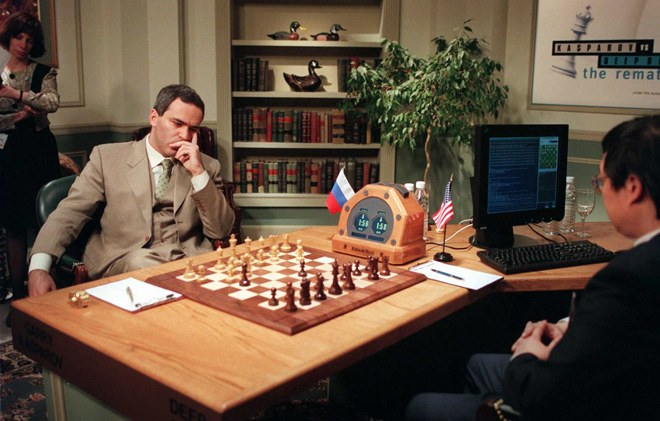
\includegraphics[width=0.8\textwidth]{images/estadodelarte/ai/deepblue-vs-kasparov}
	\centering
	\caption{El Gran Maestro de ajedrez Garri Kaspárov (izquierda) enfrentándose al ordenador Deep Blue}
\end{figure}

Estos programas suelen hacer uso de versiones muy especializadas de dos algoritmos de inteligencia artificial: Los Algoritmos de Búsqueda y el Aprendizaje automático.
\begin{itemize}
\item Un \textbf{Algoritmo de Búsqueda} es aquél algoritmo diseñado para recuperar información almacenada en una estructura de datos. Cuando se aplican a juegos, se suele emplear una versión concreta llamada Algoritmo Minimax, en el cual se trata de construir la secuencia de acciones que aseguran la victoria. Para ello, se construye una estructura en árbol con las distintas acciones que la máquina y su oponente pueden realizar donde el algoritmo pueda buscar las acciones que maximicen sus posibilidades de victoria. 
\item El \textbf{Aprendizaje Automático} es un campo de la informática donde se estudia como dotar a los ordenadores de la capacidad de aprender, es decir, de ser capaces de desarrollar nuevos comportamientos a partir de la experiencia. Los sistemas de aprendizaje orientados a juegos realizan un gran número de partidas o estudian partidas previas para poder encontrar patrones de comportamiento que les permitan ganar al juego en cuestión.
\end{itemize}

\subsection{IA Aplicada a Videojuegos: Contexto Actual}
La Inteligencia artificial aplicada a videojuegos difiere en varios puntos a su aplicación habitual en el campo de los juegos que hemos visto en el apartado anterior. La principal diferencia es el tipo de problema que se intenta resolver utilizando inteligencia artificial en cada una de las ramas: en la Inteligencia Artificial aplicada a jugar a juegos se busca obtener un sistema capaz de jugar de manera óptima, sin embargo, en la Inteligencia Artificial orientada a videojuegos lo que se busca es crear sistemas con los que el jugador pueda interaccionar y mejorar su experiencia de juego. Esta diferencia de objetivos hace que la Inteligencia Artificial no se aplique únicamente a la creación de oponentes virtuales, sino también al modelado del comportamiento de Personajes No Jugadores y a la Generación Procedimental de Contenido\cite{ai_and_games}.

En el ámbito de los videojuegos, a la Inteligencia Artificial que interacciona con el juego como un jugador más suele llamarse "Bot". Estos bots predominan en juegos competitivos donde es necesario un oponente con un grado de inteligencia elevado para suponer un reto al jugador, como los juegos de estrategia, los juegos de lucha o los juegos de disparos en primera persona. Debido al elevado coste de desarrollar una Inteligencia Artificial potente para estos juegos, por no hablar de la potencia requerida para ejecutarla, en la mayor parte de los videojuegos la Inteligencia Artificial "hace trampas", juega teniendo acceso una serie de ventajas que los jugadores humanos no tiene. Estos sistemas podrían, por ejemplo, acceder a información oculta del jugador (como la posición o recursos) a la hora de planificar estrategias o dispondrían de más y mejores recursos que sus adversarios. 

En la mayoría de los juegos, la Inteligencia Artificial no se dedica al modelado de bots como los descritos anteriormente, sino que lo más común es que se utilice para controlar el comportamiento de Personajes no Jugadores, o NPCs (siglas inglesas de Non-Player Character). Estos pueden tener comportamientos muy variados dependiendo de su papel en el juego: pueden actuar como adversarios, servir de ayuda para el jugador, formar parte de un puzle, contar una historia o simplemente formar parte del trasfondo de la acción. En el diseño de NPCs, lo que se busca son dos cosas: crear una Ilusión de Inteligencia, de forma que los jugadores crean que el NPC es un ser inteligente, aunque sea controlado por un código muy sencillo, y, en especial con adversarios, que sea predecible, de forma que el jugador pueda desarrollar estrategias para enfrentarse/interaccionar con ellos.

\begin{figure}[h]
	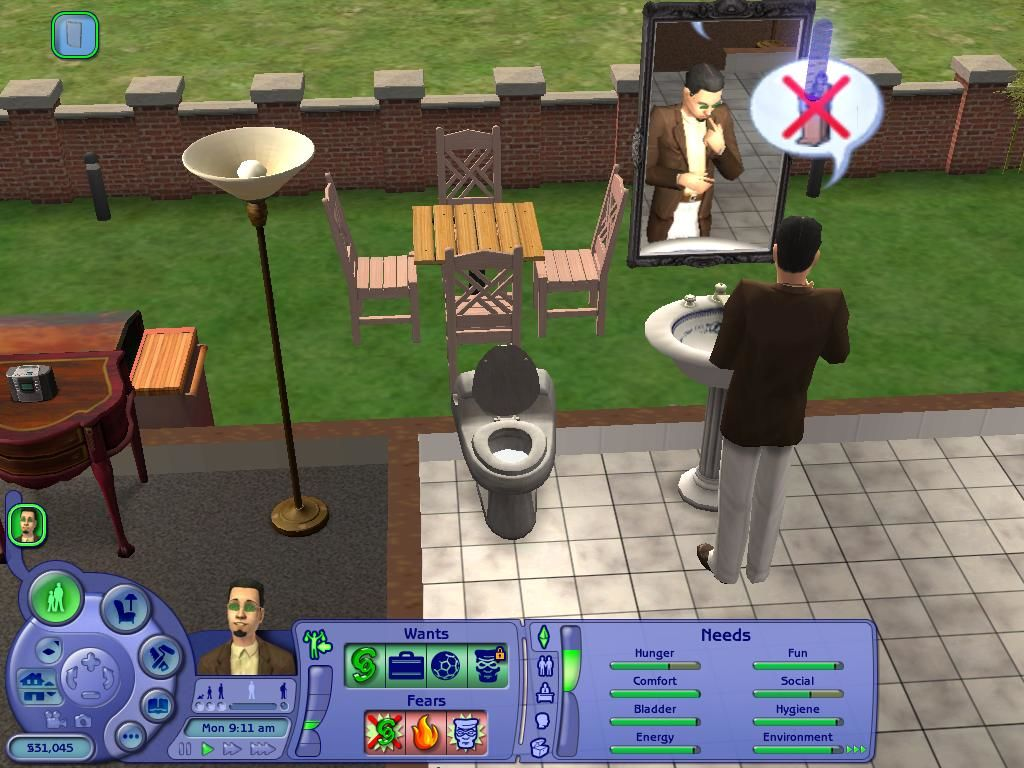
\includegraphics[width=0.8\textwidth]{images/estadodelarte/ai/sims-captura}
	\centering
	\caption{En Los Sims (Maxis, 2000-2014), los personajes pueden tomar decisiones basándose en sus gustos y necesidades.}
\end{figure}

La otra aplicación principal en los videojuegos es la Generación Procedimental de Contenido. La generación Procedimental de Contenido es el nombre que reciben los métodos que permiten generar el contenido de un juego de forma automática o con solo un mínimo de intervención humana. Actualmente, la mayor parte de los juegos que hacen uso de la generación procedimental la utilizan para la creación automática de mapas o niveles o para la creación de objetos. La generación procedimental de contenido puede utilizarse tanto como una herramienta durante el desarrollo, que serviría para generar contenido que luego sería refinado por los desarrolladores; o podría formar parte del juego final, generando nuevo contenido al gusto del jugador de forma automática.

\begin{figure}[h]
	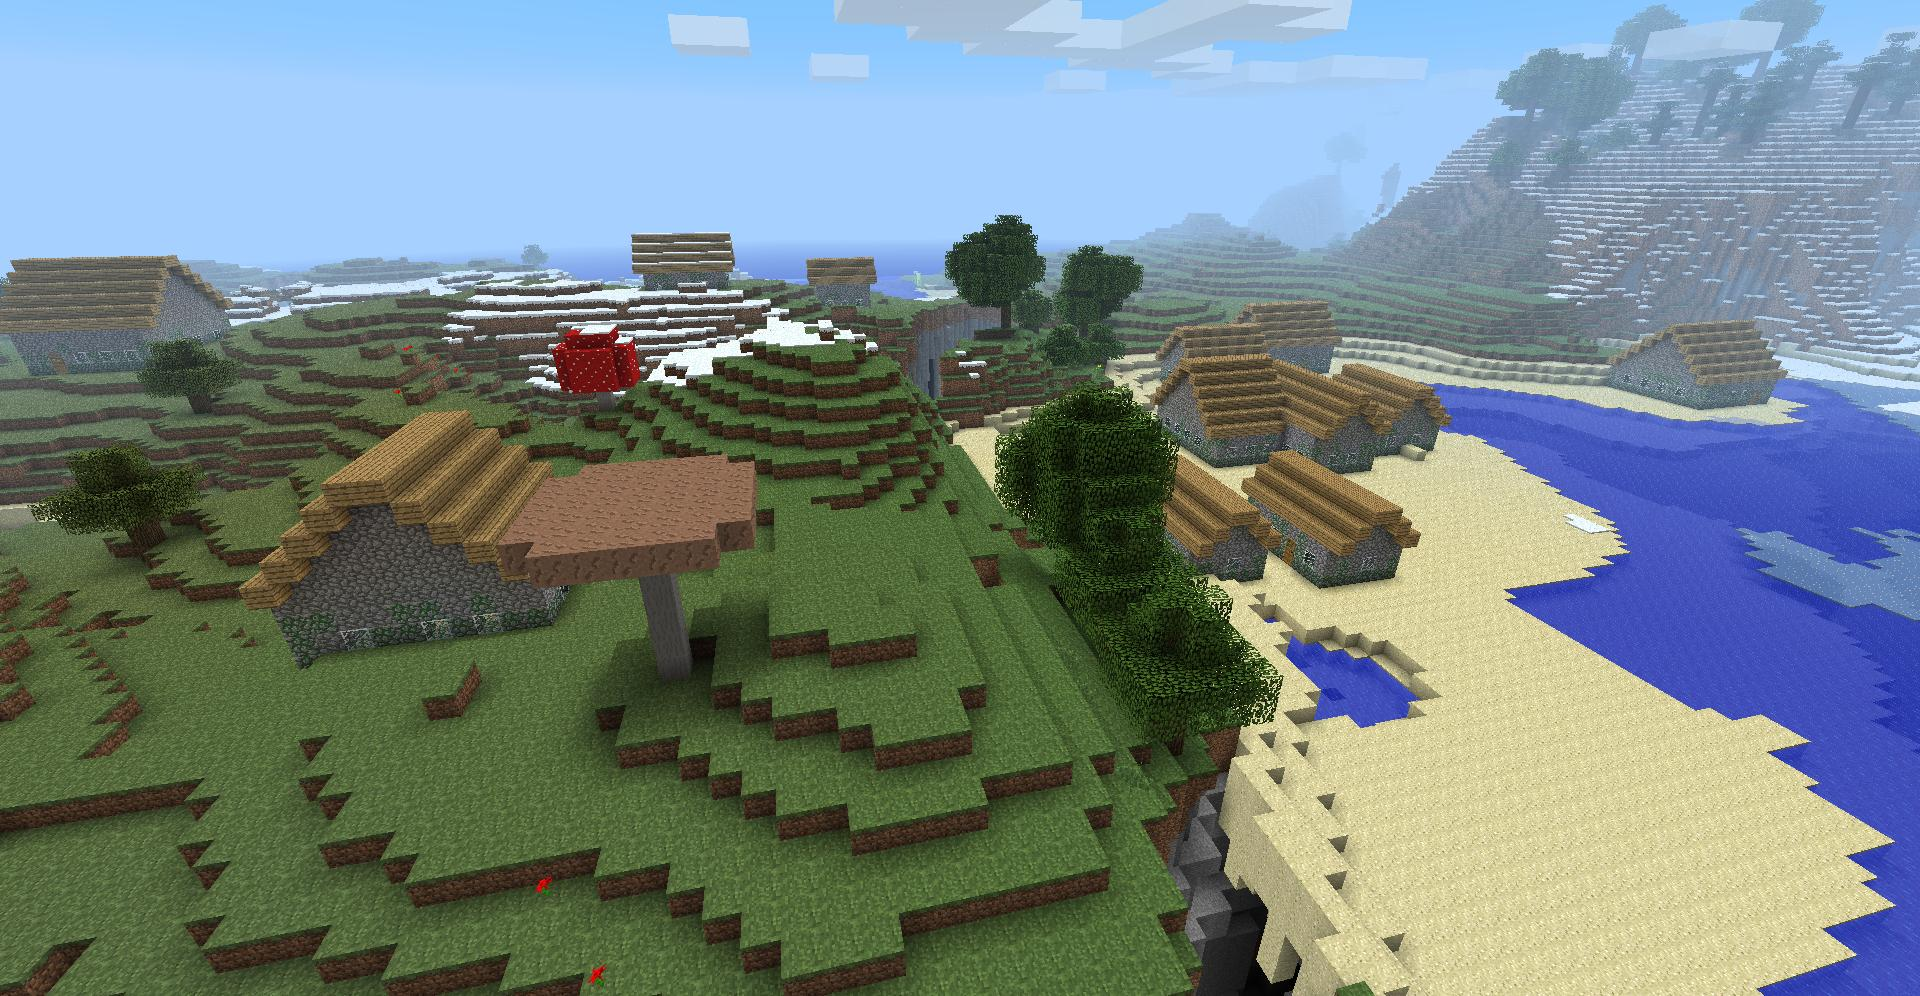
\includegraphics[width=0.75\textwidth]{images/estadodelarte/ai/minecraft}
	\centering
	\caption{Minecraft (Mojam, 2009) es un ejemplo claro de generación procedimental de terrenos.}
\end{figure}


\subsection{Futuros campos de aplicación}
La Inteligencia Artificial orientada a juegos evoluciona de manera paralela a los propios videojuegos, que viven ahora más que nunca una época dorada debido al aumento constante tanto en popularidad y prestigio, lo que supone una mejora tanto en la potencia de las máquinas que los ejecutan como en las técnicas que se utilizan en su desarrollo. Esta situación cambiante ha causado la aparición de nuevos problemas que se esperan poder solucionar con el uso de técnicas de inteligencia artificial.\cite{ai_and_games} A continuación mencionaremos algunos de los futuros campos de aplicación de las técnicas de inteligencia artificial:

Una las posibles aplicaciones de la Inteligencia Artificial es la de realizar \textbf{Testing} de juegos. El programa jugaría a los juegos en busca de fallos tanto informáticos como de diseño (como problemas de balanceo o maneras de hacer trampas en el juego) de forma automatizada, ahorrado una gran cantidad de trabajo a los desarrolladores. Aunque ya existen herramientas que ofrecen una forma rudimentaria de testing automático, aun es necesario mejorar aspectos como la categorización de los errores encontrados.

La \textbf{Minería de Datos de Juego} es otro uso prometedor de la Inteligencia Artificial. Se trata de una técnica alternativa al testing habitual de juegos en la que se recolecta y analiza la información de comportamiento de la base de jugadores de un juego dado con el fin de mejorar dicho juego\cite{ai_revisited}. Esta técnica se ha popularizado gracias a la proliferación de juegos con un fuerte componente online que facilita la recogida de datos. Sin embargo los volúmenes de datos con los que se trabaja son tan masivos que los algoritmos de mineria de datos actuales no son capaces de analizarlos completamente \cite{ai_revisited}.

La Dirección de Juegos consiste en una Inteligencia Artificial que modifica eventos del juego en tiempo real basándose en las reacciones de los jugadores con acciones tales como modificar la dificultad, reproducir música y sonido o modificar el entorno con tal de mejorar la experiencia del jugador. Actualmente, los juegos que mejor ha implementado un sistema con esta propiedad es la saga Left 4 Death de Valve\footnote{http://www.l4d.com/blog/}. Se trata de una rama con mucho potencial que aún no ha sido explorado completamente.

Finalmente, una tarea de gran importancia para los juegos online, a pesar de no formar parte de los juegos en si, es la motorización de los chats. El gran volumen de mensajes que se envían a través de los chats de los juegos online más populares hace que sea imposible la moderación manual, lo que crea un entorno de juego toxico para los jugadores. Compañías como Riot (creadora del popular MOBA League of Legends) están empezando a utilizar algoritmos de aprendizaje automático para entrenar sistemas para detectar y eliminar los mensajes inapropiados de los chats \cite{toxic_wow}.

\begin{figure}[h]
	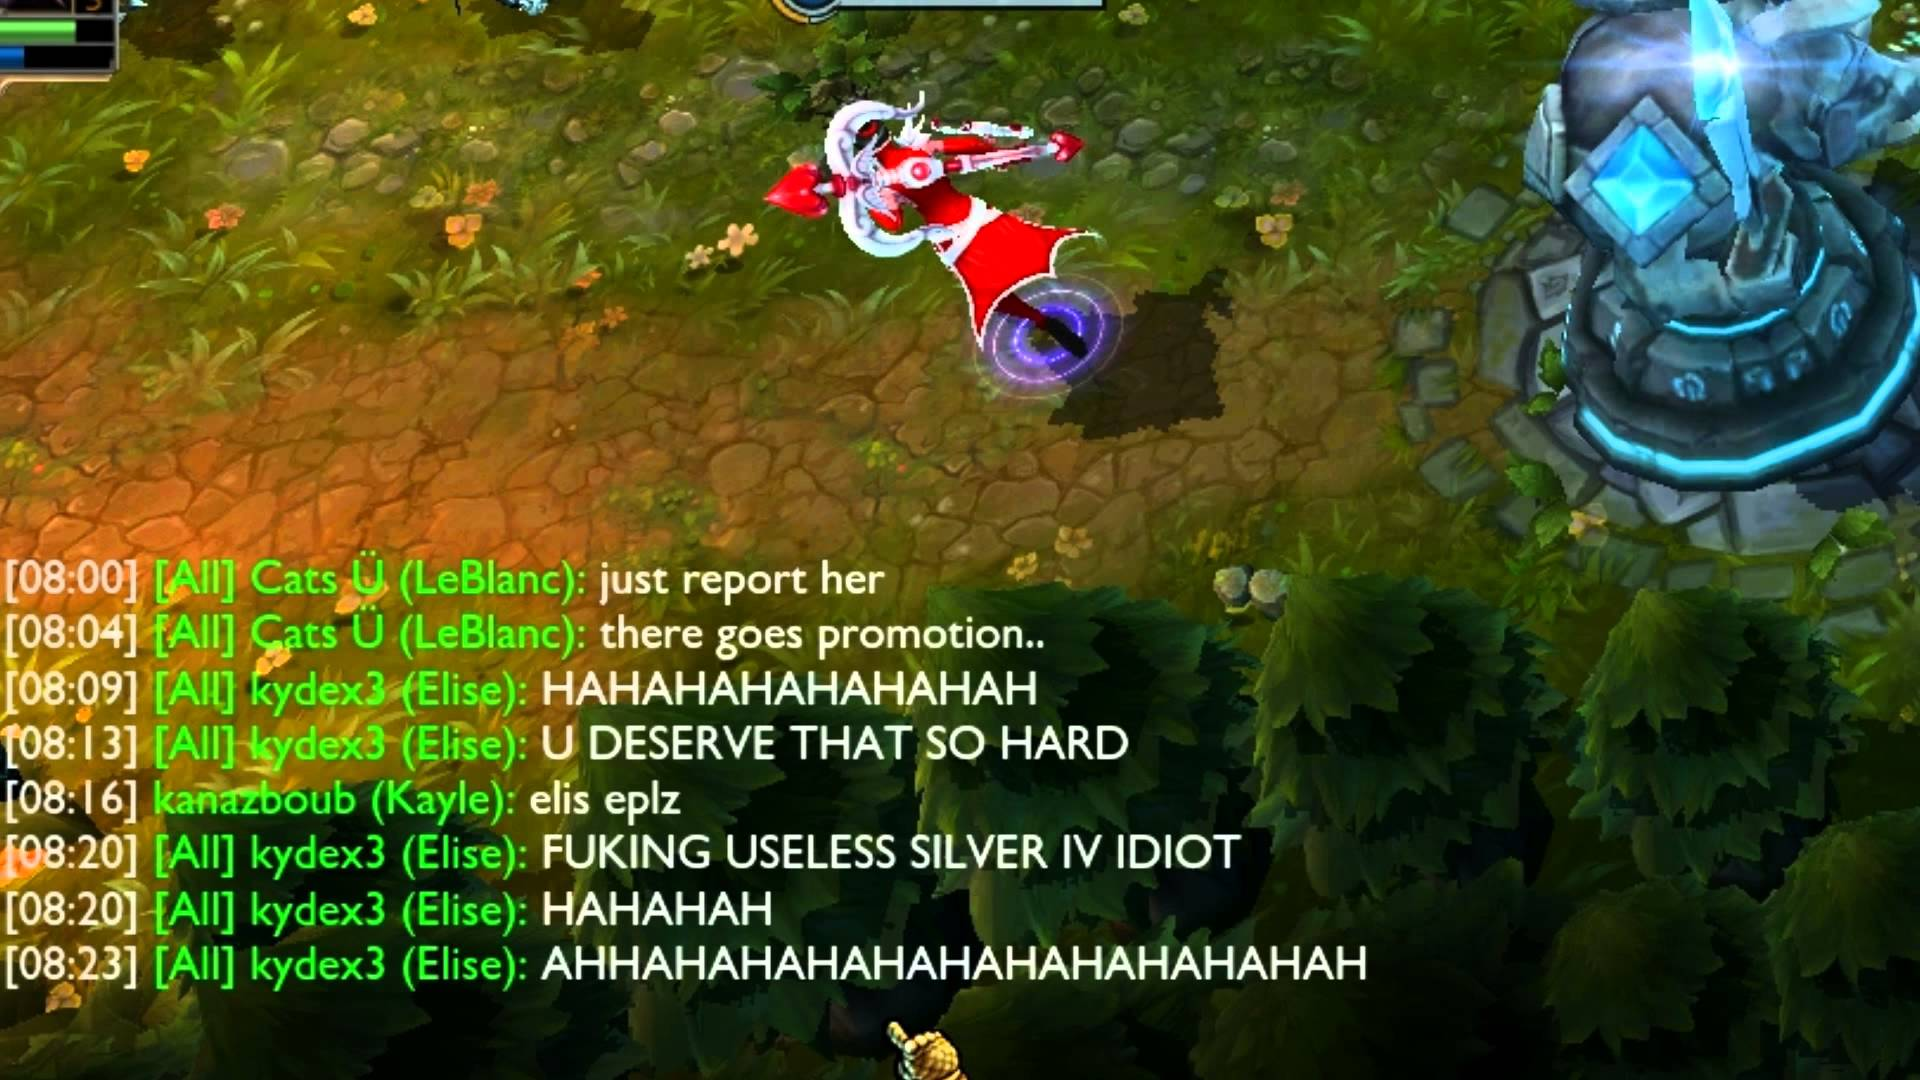
\includegraphics[width=0.45\textwidth]{images/estadodelarte/ai/lol-toxic-capture}
	\centering
	\caption{Ejemplo de comportamiento tóxico en League of Legends(Riot Games, 2009).}
\end{figure}
